\documentclass[12pt, a4paper]{article}

% ==================== Preamble ====================
\usepackage[fontset=windows]{ctex}
\usepackage{amsmath, amsfonts, amssymb}

% Western font: Times New Roman (CJK heading fonts are 黑体 by ctex default)
\setmainfont{Times New Roman}
\usepackage{graphicx}
\usepackage{caption}
\usepackage{subcaption}
\usepackage{booktabs}
\usepackage{geometry}
\geometry{left=1.8cm, right=1.8cm, top=1.8cm, bottom=1.8cm}
\usepackage{hyperref}
\hypersetup{
    colorlinks=true,
    linkcolor=blue,
    filecolor=magenta,
    urlcolor=cyan,
    citecolor=black,
}
\usepackage{xcolor}
\usepackage{tikz}
\usetikzlibrary{shapes.geometric, arrows.meta, positioning, calc}
\usepackage{tabularx}
\usepackage{array}
\usepackage{float}

\newcolumntype{L}{>{\raggedright\arraybackslash}X}

\setlength{\parindent}{1.2em}
\setlength{\parskip}{0.1em}

\renewcommand{\abstractname}{\textbf{摘要}}

% ==================== Body ====================
\begin{document}

% Compact title on page 1
{\centering
{\LARGE \heiti 面向不同车型的2.5D野外地形风险感知路径规划}\\[0.3ex]
{\Large \heiti 基于机器学习与搜索算法的双向嵌套设计}\\[1ex]
{\normalsize 东北大学自动化强基班 《人工智能》与《机器学习与模式识别》综合课程作业}\\[0.5ex]
{\normalsize 团队成员：崔瑞航、李佳阳、刘动 \quad 指导教师：陈东岳}\\[0.5ex]
\par}

\begin{abstract}
在野外复杂的2.5D地形中，传统仅依赖距离的路径规划方法难以适应不同车辆的物理通行能力差异。本设计提出了一种融合机器学习与智能优化搜索的路径规划架构：外层引入带有物理先验的风险约束A*算法，内层采用粒子群优化对CNN+MLP多任务风险预测模型进行拓扑与参数寻优。结合Gazebo物理仿真生成的高保真数据集以及ML+Geometric Guard保底机制，方案成功实现了同一复杂地形下针对不同车辆参数的自适应、低风险差异化规划。实验表明，该架构大幅降低了越野翻车和托底风险，显著提升了复杂非结构化环境下的规划成功率与系统鲁棒性。
\end{abstract}

\vspace{-0.5em}

\section{问题背景与形式化定义}

\subsection{应用背景与工程价值}
在野外救援、农业勘探与星际巡查等复杂自动化场景中，移动机器人常面临崎岖、非结构化的2.5D地形。传统路径规划算法通常将车辆抽象为二维平面上的质点，仅以几何距离作为优化目标。Gu与Cao\cite{gu2011path}率先提出将高程信息纳入A\*搜索的边代价中，形成了2.5D A\*这一经典基线。然而该方法仍将机器人视为无尺寸质点，未考虑车型差异带来的物理风险。在平坦室内环境中这一假设是合理的，但在野外地形下，相同的地形对具有不同轴距、轮径和底盘高度的车辆，其面临的侧翻、托底和打滑等物理风险截然不同。

若仅将2.5D高程图的欧氏距离作为路径代价，极易将车辆引向距离虽短却极度危险的区域。为此，本课题提出了一种车型参数化且具备物理风险感知的约束A*路径规划方案，并引入机器学习与智能优化搜索的双向嵌套架构，实现对未知非线性动态风险的精准拟合与规划应用。

\subsection{问题形式化定义}
将野外环境表示为带有物理属性的全局2.5D栅格地图 \(M=\{H(i,j), \mu(i,j)\}\)，其中 \(H\) 为高程，\(\mu\) 为地面摩擦系数。不同于传统2D规划，本课题在状态与动作空间中引入了车辆运动学与几何约束：

\begin{itemize}
    \item \textbf{状态空间 \(\mathcal{S}\)}：状态定义为 \(s=(i, j, k)\)，其中 \((i,j)\) 为车辆中心所在的栅格坐标，\(k \in \{0, 1, \dots, 15\}\) 为离散化的车辆航向角。
    \item \textbf{动作空间 \(\mathcal{A}\)}：定义为一组局部运动基元 \(a = [\Delta s, \Delta \psi]\)，包含直行与不同曲率的转向。
    \item \textbf{状态转移与边 \(e\)}：定义边 \(e = (s, a, s')\) 表示车辆从状态 \(s\) 执行动作 \(a\) 到达 \(s'\) 的过渡过程。每条边不仅具有几何长度代价 \(d_e\)，更包含通过机器学习模型预测的物理交互风险 \(\hat{r}_e\)。
\end{itemize}

\textbf{规划目标与约束}：本课题不采用距离与风险简单线性加权的软惩罚方式，因为这种方式容易让短距离的优势掩盖高风险，而是将其建模为带硬约束的组合优化问题。给定起点 \(s_{start}\) 与目标区域 \(G\)，寻找一条路径 \(\pi = \{e_1, e_2, \dots, e_T\}\)，使得：

\begin{equation}
    \min_{\pi} L(\pi) = \sum_{e \in \pi} d_e
\end{equation}

且满足以下安全性硬约束：

\begin{align}
    \hat{r}_e &\le T_{edge}, \quad \forall e \in \pi \quad \text{(单步动作风险约束)} \\
    R_{max}(\pi) &= \max_{e \in \pi} \hat{r}_e \le T_{max} \quad \text{(路径最大风险约束)} \\
    R_{avg}(\pi) &= \frac{\sum_{e \in \pi} d_e \hat{r}_e}{L(\pi)} \le T_{avg} \quad \text{(路径平均风险约束)}
\end{align}

其中 \(T_{edge}, T_{max}, T_{avg}\) 为安全阈值。在此架构中，外部搜索算法需要内部机器学习模型提供精准的 \(\hat{r}_e\)，而内部模型的超参数与上述阈值又需要依赖智能搜索算法自动寻优，从而构成双向嵌套协同的需求。

%====================================================================

\section{外层设计：风险约束A*与机器学习启发}

外层架构中，A*搜索算法通过调用已训练好的内层机器学习模型，获取局部状态转移的物理风险估计。该风险值既作为启发信息引导搜索方向，也用于剪除高风险分支，从而大幅压缩无效的搜索空间。

\subsection{风险预测模型输入与架构}
传统评估方法仅考察单一栅格的状态，而物理风险实际上发生在车身扫掠整个动作区域的动态过程中。因此，将机器学习模型的输入设计为四元组 \(X = (X_{map}^{s,a}, \theta_v, a, \mu)\)：

\begin{enumerate}
    \item \textbf{局部地形特征 \(X_{map}^{s,a} \in \mathbb{R}^{31 \times 31 \times 6}\)}：以车辆当前位置为中心，沿车身航向截取的局部高程、纵/横向坡度、粗糙度，以及车身掩码和动作扫掠掩码。
    \item \textbf{车辆参数向量 \(\theta_v \in \mathbb{R}^{12}\)}：包含车长、车宽、轮径、底盘高度、质心高度等物理参数。
\end{enumerate}

模型采用\textbf{CNN + MLP 双分支融合架构}：CNN提取 \(X_{map}\) 的空间几何特征，MLP提取参数特征，融合后输出多任务物理风险 \(\hat{y} = [\hat{y}_{fail}, \hat{q}_{roll}, \hat{q}_{pitch}, \hat{q}_{slip}, \hat{q}_{lift}, \hat{p}_{bottom}, \hat{p}_{stuck}]\)，涵盖侧翻、俯仰、打滑、托底等多维危险概率。多维风险通过权重向量 \(w\) 融合为单一标量边风险 \(r_{ml}\)。

\subsection{基于 ML+Guard 的鲁棒融合机制设计}
在实际工程实现与Gazebo物理仿真数据收集过程中发现：为保证仿真引擎物理接触约束的稳定性，数据收集阶段的稳定性门控客观上过滤掉了部分极端非平坦地形，导致机器学习模型在面临断崖等极高频凸起时可能因分布外数据而低估风险。

为保证系统在任意未知地图上的绝对安全性与可解释性，本方案在外层A*规划的代价评估环节提出并实现了\textbf{ML + Geometric Guard}融合机制，即物理先验保底机制：

\begin{equation}
    r_{plan} = (1-\lambda_g) \, r_{ml} + \lambda_g \cdot \max(r_{ml}, r_{manual})
\end{equation}

其中 \(r_{manual}\) 为基于局部扫掠区域坡度与粗糙度的人工保守风险值，\(\lambda_g\) 为保底权重，本方案取 \(\lambda_g = 0.5\)。该设计既保留了ML模型对不同车型在复杂地形上的精细分辨力，又在ML可能失效的极端几何突变处提供了严格的安全性下界，使A*算法的硬约束剪枝逻辑更加鲁棒。

%====================================================================

\section{内层设计：PSO智能优化模型}

上述机器学习模型的网络结构、损失函数分配比例以及规划层的安全阈值均具有高度的非线性与耦合性，难以通过经验法则或简单网格搜索获得全局最优解。因此，内层采用\textbf{粒子群优化算法}对模型超参与规划阈值进行联合寻优。

\subsection{粒子编码与搜索空间设计}
每个粒子 \(\mathbf{z}\) 代表一组完整的模型-规划配置，其编码维度共计20维，涵盖三大类：

\begin{enumerate}
    \item \textbf{网络结构与训练参数}：CNN各层通道数组合、隐藏层神经元个数、Dropout比例、学习率、权重衰减系数。
    \item \textbf{多任务损失权重}：对分类失败、托底、卡住、回归误差的损失函数权重 \(\lambda_f, \lambda_b, \lambda_s, \lambda_r\) 进行自动分配，解决多任务学习中梯度不平衡问题。
    \item \textbf{风险融合权重与规划阈值}：多维风险融合成标量的7维权重向量 \(w_i\)，以及外层A*的硬约束阈值 \(T_{edge}, T_{max}, T_{avg}\)。
\end{enumerate}

\subsection{复合适应度函数设计}
常规的自动机器学习方法仅以验证集损失函数作为优化目标，但本课题的最终目的是服务于路径规划，模型预测精度的提升未必等同于规划成功率的提升。因此，在内层PSO的评价阶段引入了代理规划评估，即在小型验证地图上实际运行A*规划来反馈模型质量，并将适应度函数设计为如下复合指标：

\begin{equation}
    Fitness = \text{AUC}_{fail} + \alpha_1 \cdot \text{Recall}_{fail} - \alpha_2 \cdot \text{MAE}_{risk} - \alpha_3 \cdot t_{infer} + \beta_1 \cdot \text{PlanSR} + \beta_2 \cdot \text{OracleSR}
\end{equation}

式中，前三项评估模型在验证集上的离线辨识精度与查全率，优先惩罚风险漏报情况；\(t_{infer}\) 惩罚过度庞大的网络结构以保证A*的节点扩展效率。\(\text{PlanSR}\) 代表将该粒子生成的模型投入小型验证地图进行实际A*规划的成功率，\(\text{OracleSR}\) 代表模型决策与真实物理标签的一致性。通过这一复合适应度函数，PSO并非盲目地调整超参数，而是真正实现了由搜索结果反馈至模型结构的闭环优化。

\section{双向嵌套协同架构：耦合机制与理论分析}

在复杂的工程场景中，单一的搜索算法或机器学习模型均存在各自的性能瓶颈：搜索算法缺乏物理先验，而机器学习模型在缺少针对性结构设计时难以直接对接离散的组合优化任务。本方案的核心创新在于构建了一个数据流与控制流高度解耦、优化目标又深度耦合的双向嵌套协同架构。

\subsection{整体架构与交互逻辑}

图~\ref{fig:architecture} 展示了全流程协同机制，系统划分为三大逻辑域：物理数据引擎、内层智能搜索和外层风险约束搜索。

\begin{figure}[htbp]
    \centering
    \resizebox{\textwidth}{!}{
    \begin{tikzpicture}[>=latex, thick, scale=0.72, transform shape]
        \tikzstyle{box} = [rectangle, draw=black!60, rounded corners, text centered, minimum height=0.9cm]
        \tikzstyle{dataBox} = [box, fill=gray!15, text width=2.3cm]
        \tikzstyle{psoBox} = [box, fill=blue!10, text width=4.0cm]
        \tikzstyle{mlBox} = [box, fill=green!10, text width=4.0cm]
        \tikzstyle{proxyBox} = [box, fill=orange!10, text width=2.8cm]
        \tikzstyle{astarBox} = [box, fill=red!10, text width=5.8cm]

        \node[dataBox] (gazebo) at (-6.5, 2.0) {\textbf{Gazebo物理引擎}\\[0.1ex]\scriptsize 提取局部打滑/碰撞};
        \node[dataBox] (data) at (-6.5, -1.5) {\textbf{多模态仿真数据集}\\[0.1ex]\scriptsize $(X_{map}, \theta_v, a, \mu) \rightarrow y$};

        \node[psoBox] (pso) at (0, 2.0) {\textbf{内层智能搜索 (PSO)}\\[0.1ex]\scriptsize 种群: [网络超参, 损失/融合权重, 安全阈值]};
        \node[mlBox] (ml) at (0, -1.5) {\textbf{多任务风险评估模型}\\[0.1ex]\scriptsize CNN+MLP 预测 7 维动态风险};

        \node[proxyBox] (proxy) at (6.5, 2.0) {\textbf{代理规划评估}\\[0.1ex]\scriptsize Proxy A* 小规模验证};

        \node[astarBox] (astar) at (0, -4.5) {\textbf{外层智能搜索 (风险约束 A*)}\\[0.1ex]\scriptsize ML+Geometric Guard 融合机制与全局寻优};

        \draw[->] (gazebo) -- node[right] {\scriptsize 生成时序标签} (data);
        \draw[->] (data) -- node[above] {\scriptsize 提供训练数据} (ml);

        \draw[->] ([xshift=-1.2cm]pso.south) -- node[left, align=right] {\scriptsize 结构超参 $\Theta$\\ \scriptsize 损失权重 $\lambda$} ([xshift=-1.2cm]ml.north);
        \draw[->, dashed, draw=black!60] ([xshift=1.2cm]ml.north) -- node[right, align=left] {\scriptsize 验证集回归 Loss} ([xshift=1.2cm]pso.south);

        \draw[->] (pso.east) -- node[above] {\scriptsize 安全阈值 $T$} (proxy.west);
        \draw[->] (ml.east) -| node[above, near start] {\scriptsize 模型预测风险 $\hat{r}_e$} (proxy.south);

        \draw[->, rounded corners, draw=blue!80!black, line width=1.0pt]
            (proxy.north) |- ++(0, 0.7) -| node[above, near start] {\textbf{返回复合 Fitness}} (pso.north);

        \draw[->] ([xshift=-1.2cm]astar.north) -- node[left, align=right] {\scriptsize 候选搜索动作\\ \scriptsize 姿态 $(s, a)$} ([xshift=-1.2cm]ml.south);
        \draw[->] ([xshift=1.2cm]ml.south) -- node[right, align=left] {\scriptsize 返回智能风险启发\\ \scriptsize $r_{plan} \Rightarrow$ 用于剪枝} ([xshift=1.2cm]astar.north);

        \draw[->, dashed, draw=purple!80!black, line width=1.0pt, rounded corners]
            (pso.east) -- (9.2, 2.0) -- node[right, align=left] {\scriptsize 部署全局最优模型 $f_{\Theta^*}$\\ \scriptsize 与最佳阈值 $T^*$} (9.2, -4.5) -- (astar.east);
    \end{tikzpicture}
    }
    \caption{机器学习与搜索双向嵌套协同架构}
    \label{fig:architecture}
\end{figure}

根据图~\ref{fig:architecture}：Gazebo 引擎生成高保真数据集，导入内层 CNN+MLP 网络进行特征提炼。内层 PSO 通过改变粒子位置重塑 ML 模型的网络结构和训练法则，代理 A* 接收模型输出并在小规模沙盒上规划，将不可导的规划结果转化为 Fitness 标量反馈给 PSO。外层 A* 将节点探索请求 \((s,a)\) 下发给 ML 模型，ML 模型凭借泛化能力为每条扩展边赋予风险成本，将搜索转变为安全导向探索。

\subsection{协同优化的理论优势}

\textbf{1. 突破规则启发函数的能力上限——机器学习赋能搜索。}传统2.5D A*仅利用几何高度差作为代价，本质上属于静态惩罚。然而地形对车辆造成的侧翻、打滑等风险是高度非线性的，取决于轴距 \(l\)、轮距 \(b\) 与当前姿态。外层引入经 PSO 优化的 ML 模型后，搜索树的扩展获得了物理引擎级别的先验知识。对于超过最优阈值 \(T^*_{edge}\) 的候选边，A*可提前剪枝，从而避免传统搜索算到死胡同才回溯的维度灾难。针对 ML 在分布外数据上可能失效的问题，本方案在耦合边界处增加了 Geometric Guard 手工几何保底机制，保证了在极端未见地形中搜索代价的下界安全性。

\textbf{2. 解决模型参数的不可微寻优难题——搜索反哺机器学习。}内层面临的核心矛盾在于：机器学习模型在验证集上的分类损失最低，并不等同于外层路径规划的成功率最高。由于 A* 的寻优过程和硬约束截断逻辑完全离散且不可微，无法通过梯度下降法向网络结构传递反馈。内层的 PSO 算法恰好弥补了这一短板：通过零阶黑盒优化，PSO 在验证集误差的基准上，直接将代理规划成功率纳入全局适应度函数。这种反哺机制促使 ML 模型不再片面追求微小的回归误差，转而学习那些能切实提高车辆存活率的决策边界。

\section{仿真实验设计与结果分析}

实验环境：Ubuntu 24.04，ROS 2 Jazzy + Gazebo Sim 8.11（Bullet-Featherstone 物理引擎），PyTorch 2.11（CUDA 13），Intel Core i7-13700，NVIDIA RTX 4060。为验证双向嵌套协同架构的有效性，本方案完成了从底层数据生成、模型内层调优到外层路径规划的全链路闭环验证。

\subsection{多模态仿真数据集与物理风险标定}
本课题摒弃了缺乏物理意义的人工代价，采用 Gazebo/ros\_gz 高保真物理引擎构建了包含 20,000 个局部动作过渡的交互数据集。引擎中完整配置了车辆的碰撞体、悬挂接触传感器与里程计。在程序随机生成的参数化2.5D地形上执行离散动作，系统自动提取侧翻、俯仰、托底、车轮悬空及打滑等多维物理风险。仿真标定真实反映了地形—车辆—动作三者的非线性交互耦合。

\begin{figure}[htbp]
    \centering
    \begin{minipage}{0.46\textwidth}
        \centering
        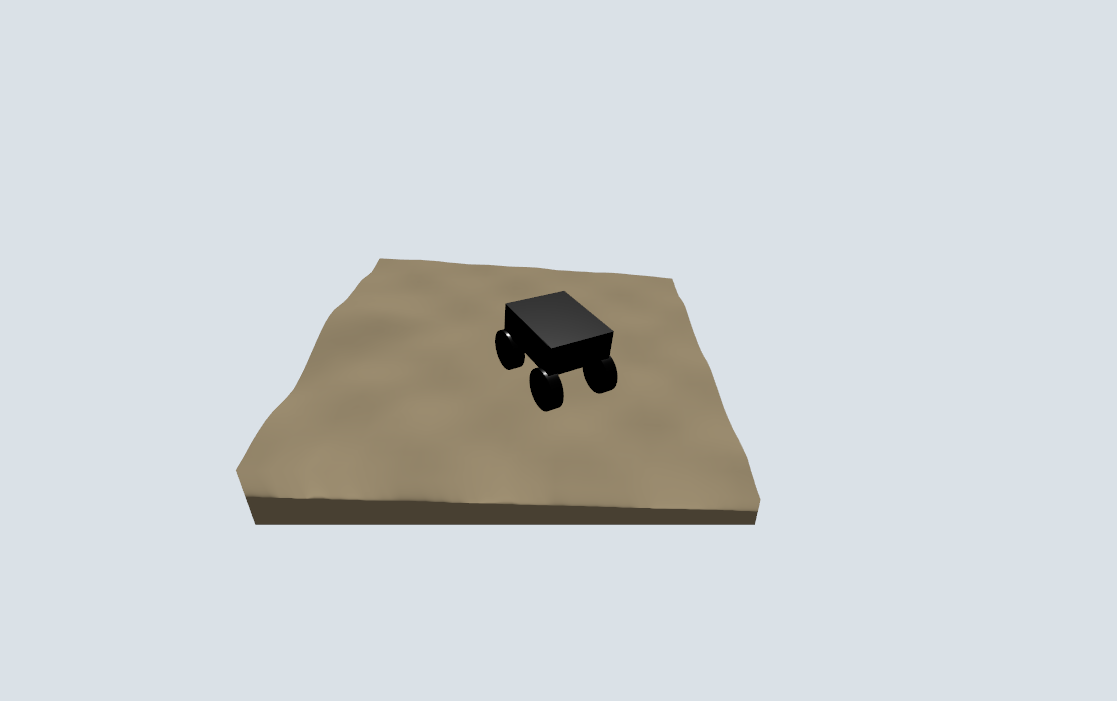
\includegraphics[width=\linewidth]{figures/gazebo_sample_safe.png}
        \caption*{大型山地车右小转，判定为安全}
    \end{minipage}\hfill
    \begin{minipage}{0.46\textwidth}
        \centering
        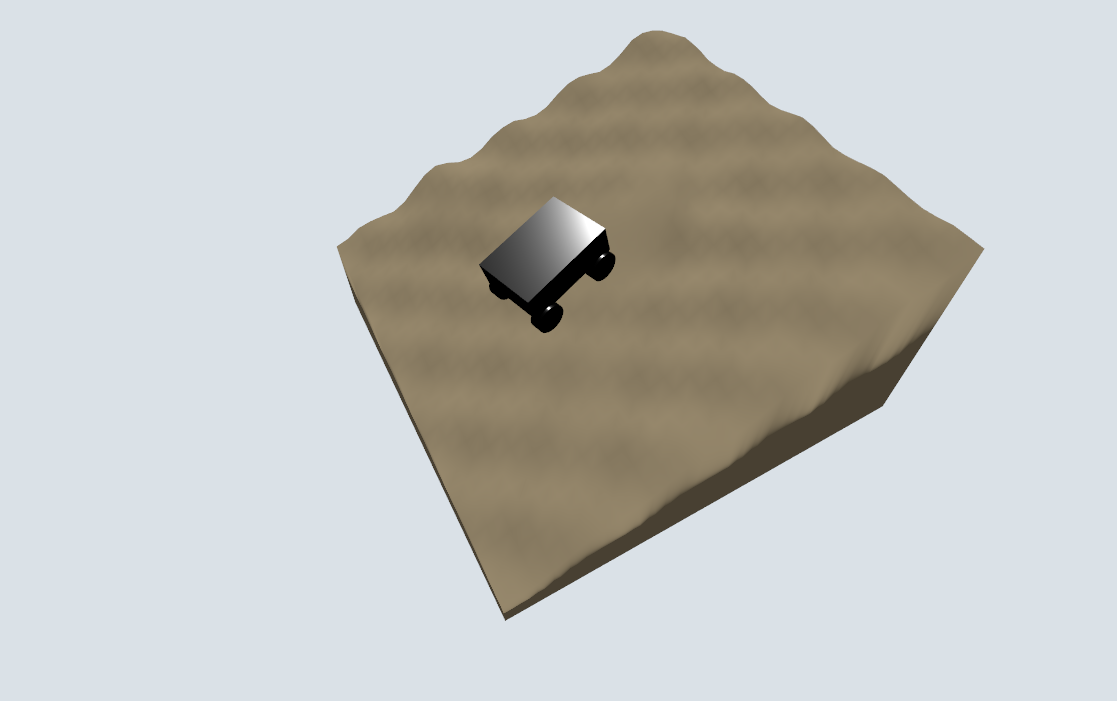
\includegraphics[width=\linewidth]{figures/gazebo_sample_critical.png}
        \caption*{标准越野车直行上坡，判定为临界危险}
    \end{minipage}
    \caption{基于Gazebo物理引擎的局部动作仿真与多维风险标签自动提取}
    \label{fig:dataset_samples}
\end{figure}

图~\ref{fig:dataset_samples} 展示了数据集中两个典型的物理仿真切片。左图对应大型山地车，尺寸为 85$\times$55 cm、质量 20 kg，在凸起障碍地形上执行右小转动作，地面为草地软土，摩擦系数约 0.5。凭借大轮径与高底盘，车轮未发生悬空且底盘无碰撞，系统判定为极度稳定，标签为安全。右图对应标准越野车，尺寸为 65$\times$45 cm、质量 14 kg，在斜坡叠加凸起地形上执行直行动作，地面同为草地软土。上坡时轴荷重分配发生突变，前轮压过凸起时短暂悬空，悬空风险骤升且伴随轻微打滑，车辆处于失控边缘，标签为临界。这类细粒度的多维物理交互构成了内层机器学习模型的训练基础，使模型具备了替代传统人为几何代价的真实物理先验能力。

\subsection{定量分析：双向嵌套与 ML+Guard 的消融验证}
为证明内层 ML 模型及其融合机制在外层规划中的核心价值，我们在 27 张未知测试地图上针对 3 种车型共 81 个规划任务进行了消融对比实验。约束条件统一为：单步动作风险阈值 \(T_{edge}=0.70\)，路径最大风险阈值 \(T_{max}=0.90\)，平均风险阈值 \(T_{avg}=0.49\)。

实验设置了五组对比方法。Baseline 1 为原始 2.5D A\*，源自 Gu 与 Cao 提出的经典方法\cite{gu2011path}，仅以三维欧氏距离作为边代价，完全忽略车辆物理参数与通行风险，代表传统方案的上界。Baseline 2 在距离代价上附加基于局部扫掠区域坡度与粗糙度的手工线性惩罚项，用于验证纯几何规则的局限性。Baseline 3 将 PSO 优化后的 ML 模型预测风险以线性加权形式融入代价函数，证明仅靠软惩罚难以彻底规避高风险区域。Guard Only 采用与 Baseline 2 相同的手工几何风险计算，但以 Proposed 相同的硬约束框架执行搜索，用于剥离 ML 模型在硬约束下的净贡献。本方案 ML+Guard 则是在 ML 风险硬约束基础上叠加手工几何保底机制。

实验结果如表~\ref{tab:ablation} 所示。

\begin{table}[htbp]
    \centering
    \caption{路径规划消融实验对比，共 81 个测试任务}
    \label{tab:ablation}
    \begin{tabular}{@{} l l c c c @{}}
        \toprule
        \textbf{方法} & \textbf{代价/约束类型} & \textbf{成功率} & \textbf{平均绕路比} & \textbf{最大风险均值} \\
        \midrule
        原始 2.5D A* & 仅三维欧氏距离 & 0.0\% & 1.00 & 0.885 \\
        手工代价 A* & 距离 + 几何粗糙度软惩罚 & 22.2\% & 1.03 & 0.542 \\
        ML 风险 A* & 距离 + ML 预测风险软惩罚 & 38.5\% & 1.08 & 0.410 \\
        纯几何规则硬约束 A* & 手工几何规则硬约束 & 40.7\% & 1.25 & 0.408 \\
        \textbf{本方案 ML+Guard} & \textbf{ML 复合硬约束} & \textbf{55.6\%} & \textbf{1.32} & \textbf{0.358} \\
        \bottomrule
    \end{tabular}
\end{table}

从表~\ref{tab:ablation} 可以得出：

\begin{enumerate}
    \item 采用软惩罚的方法由于代价尺度不统一，依然存在为缩短距离而强行穿越危险区域的现象，导致成功率偏低。
    \item 相较于仅依赖手工几何规则作为硬约束的方法，成功率 40.7\%，引入经 PSO 优化的多任务 ML 模型后，本方案成功率提升至 55.6\%，提升近 15 个百分点。根本原因在于手工几何规则缺乏弹性，例如对所有微小凸起一律判定为高危；而 ML 模型精确学到了特定车辆真实跨障的物理边界，从而在保持低风险的同时，解锁了大量原本被粗糙规则误杀的狭窄安全通道，最终将最大风险均值降到仅 0.358。
\end{enumerate}

\subsection{定性分析：不同车型的路径规划分化}

外层 A* 规划调用内层 ML 模型后，最直观的成果体现在同一复杂地形下，针对不同参数车辆展现出的差异化路径选择。我们选取了一处典型的散落障碍场景，对三种代表性车辆的规划路径进行对比，结果如图~\ref{fig:scene_compare} 所示。

\begin{figure}[H]
    \centering
    \begin{subfigure}{0.38\textwidth}
        \centering
        
\includegraphics[width=\linewidth, trim={1cm 1cm 1cm 1cm}, clip]{figures/custom_scattered_scene_001__urban_small__methods.png}
        \caption{小型城市车}
        \label{fig:scene_urban_small}
    \end{subfigure}
    \hfill
    \begin{subfigure}{0.38\textwidth}
        \centering
        
\includegraphics[width=\linewidth, trim={1cm 1cm 1cm 1cm}, clip]{figures/custom_scattered_scene_001__standard_offroad__methods.png}
        \caption{标准越野车}
        \label{fig:scene_standard_offroad}
    \end{subfigure}

    \vspace{-0.5cm}

    \begin{subfigure}{0.38\textwidth}
        \centering
        
\includegraphics[width=\linewidth, trim={1cm 1cm 1cm 1cm}, clip]{figures/custom_scattered_scene_001__mountain_large__methods.png}
        \caption{大型山地车}
        \label{fig:scene_mountain_large}
    \end{subfigure}

    \vspace{-0.2cm}
    \caption{同一散落障碍地形下不同车型的规划路径对比，红线为本方案}
    \label{fig:scene_compare}
\end{figure}

观察图~\ref{fig:scene_compare} 中本方案规划路径（红色实线），可以看出不同车型之间显著的路径分化。

小型城市车轮径仅 0.06 m，底盘高度 0.04 m，中央区域密集的坑洼与凸起对它而言属于高风险区。本方案模型控制 A* 算法放弃了中央路线，选择沿地图上边缘和右边缘平滑绕行，路径长度 21.4 m，平均风险仅 0.10。标准越野车和大型山地车具备较强的跨障与抗侧翻能力，本方案为它们规划了从地图左侧切入、沿底部穿行的路线，两者路径走向一致。其中大型山地车凭借更大的轮径 0.15 m 和更高的离地间隙 0.13 m，在拐角处更加紧凑，路径长度 17.5 m，略短于标准越野车的 17.7 m，平均风险均为 0.19。

相比之下，传统 2.5D A* 对三种车型都给出了一条近乎笔直的对角线，长度约 13.7 m，直接贯穿高差变化最剧烈的区域，在真实物理环境中极大概率导致翻车或托底。纯手工几何约束方法虽产生了一定弯折，但缺乏对全局风险深度的弹性判断，在小车任务中平均风险仍高达 0.28。

以上结果表明，引入 ML 模型后，系统不仅具备了对不同车型通过能力的判别能力，还通过 ML+Guard 融合机制避免了手工规则僵化带来的风险遗漏，实现了数据驱动下因车制宜的自适应规划。

\section{团队分工与总结}

\subsection{工作总结}
本综合设计围绕机器学习为搜索提供启发、搜索为机器学习提供参数寻优的双向协同要求展开，形成了从问题建模、物理仿真、模型训练到规划验证的完整闭环，主要成果体现在以下方面：

\begin{enumerate}
    \item \textbf{双向嵌套协同架构}：自主实现了内层 PSO 复合适应度寻优与外层 ML 风险约束 A*，通过代理规划评估构成反馈闭环。
    \item \textbf{基于物理仿真的高保真数据}：借助 Gazebo 物理引擎生成了 20,000 次包含侧翻、托底、打滑等真实动力学标签的交互数据，使 ML 模型具备了接近实体的风险评估能力。
    \item \textbf{ML+Guard 鲁棒融合机制}：针对仿真数据筛选引起的分布外低估问题，将数据驱动的精细判别与几何先验的安全性下界融合，提升了极端地形下的规划鲁棒性。
    \item \textbf{方法创新}：提出将 ML 风险预测作为 A\* 硬约束而非软惩罚的规划范式，避免距离优势稀释风险；设计复合适应度函数将不可微的规划成功率反馈至 PSO，实现搜索与学习的真正闭环。
\end{enumerate}

\subsection{团队分工}
本团队共 3 人，分工明确，全流程无缺失，具体分工如表~\ref{tab:contribution} 所示。

\begin{table}[htbp]
    \centering
    \caption{团队分工与完成情况}
    \label{tab:contribution}
    \small
    \begin{tabular}{p{2.2cm} p{11.2cm}}
        \toprule
        \textbf{成员} & \textbf{核心职责与实际完成情况} \\
        \midrule
        崔瑞航 &
        \textbf{核心算法开发与系统架构设计}：搭建内层 CNN+MLP 多任务风险评估模型的网络架构；设计并实现内层 PSO 搜索算法及复合适应度函数，含代理规划评估模块；实现外层带 ML+Geometric Guard 约束的 A* 算法核心逻辑；串联内外层数据流与控制流，完成耦合交互的联合调试。 \\
        \midrule
        李佳阳 &
        \textbf{物理仿真数据链与建模定义}：完成问题场景的数学形式化定义与状态/动作空间建模；基于 Gazebo/ros\_gz 搭建多模态地形生成流程；定义车辆实体物理参数，负责运行并提取 20,000 次局部动作的碰撞、打滑等标签；负责数据集的封装、验证与数据加载预处理。 \\
        \midrule
        刘动 &
        \textbf{消融实验、可视化与报告撰写}：搭建手工代价、纯 ML 风险等多种基线方法，执行大规模消融对比实验；利用 Matplotlib/PyVista 绘制二维与三维路径对比图；汇总实验数据，进行结果统计与核心结论提炼；完成综合设计报告的 \LaTeX{} 排版与答辩材料制作。 \\
        \bottomrule
    \end{tabular}
\end{table}

通过本次综合大作业，团队成员深入理解了搜索算法与机器学习模型的优势互补关系，锻炼了从工程抽象、物理仿真数据构建到算法联合寻优与系统验证的自动化复杂系统设计能力。

\newpage
\section*{附录}


\begin{thebibliography}{99}

\bibitem{gu2011path}
J.~Gu and Q.~Cao.
\newblock Path planning for mobile robot in a 2.5-dimensional grid-based map.
\newblock \emph{Industrial Robot}, 38(2):126--134, 2011.
\newblock DOI: 10.1108/01439911111122815.

\end{thebibliography}

\end{document}
